%
% Projekt: proj4.tex
% Autor:   Michal Ľaš
% Datum:   11.04.2023
% 


\documentclass[a4paper, 11pt, a4paper]{article}
\usepackage[left=2cm,text={17cm, 24cm},top=3cm]{geometry}

\usepackage[slovak, english]{babel}
\usepackage{times}
\usepackage[utf8]{inputenc}
\usepackage[T1]{fontenc}
\usepackage[hidelinks]{hyperref}
\usepackage{url}
\usepackage{graphicx}

\graphicspath{{../images/}}
%\DeclareUrlCommand\url{\def\UrlLeft{<}\def\UrlRight{>} \urlstyle{tt}}


\begin{document}


\begin{titlepage}
    \begin{center}
            \textsc{\Huge Brno University of Technology \\}
            \vspace{0.5em}
            \textsc{\huge Faculty of Information Technology \\}
        \vspace{\stretch{0.382}}
            {\LARGE Network Applications and Network Administration\,--\,Project \\ 
            \vspace{0.4em}
            \Huge DHCP-stats Manual}
        \vspace{\stretch{0.618}}
    \end{center}
    {\Large \today \hfill Michal Ľaš (xlasmi00)}
\end{titlepage}

% Table of contents
\tableofcontents
\newpage

% Body
\section{Introduction}

This introduction provides essential information necessary for comprehending the functioning of the dhcp-stats tool. 
For a thorough understanding of the complex operations of the DHCP protocol, see \cite{rfc2131}.

\bigskip

\noindent The Dynamic Host Configuration Protocol (DHCP) provides a framework
for passing configuration information to hosts on a TCP/IP network.
DHCP is providing two services:

\begin{enumerate}
    \item it is delivering host-specific configuration parameters
    \item it is assigning network addresses to its hosts
\end{enumerate}

\noindent DHCP is built on a client-server model, where designated DHCP server
is a host that allocate network addresses and deliver configuration parameters to other network hosts.\cite{rfc2131}

\noindent The number of addresses that the server can allocate is limited, therefore each DHCP server must keep records of the allocated addresses. 
In case of allocation of all the addresses the DHCP server should notify the administrator.
This is also the main purpose of \textbf{dhcp-stats} tool \ref{section:design}.


\subsection{The DHCP Packet Header}

\begin{figure}[ht]
    \begin{center}
        \scalebox{0.6}{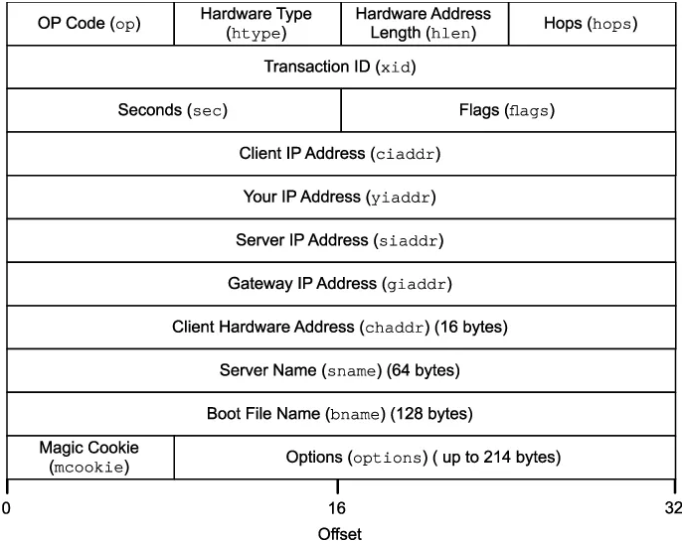
\includegraphics{../images/dhcp-packet.png}}
    \end{center}
    \caption{Structure of DHCP packet (figure from: \cite{Avocado.Aun.dhcp})}
    \label{figure:dhcp-packet}
\end{figure}


\subsection{DHCP Messages: }

\noindent\large{\textbf{DHCP discover message}}

This is the first message in DHCP communication. The client broadcasts a DHCP discover message without knowing its IP address.
The desticantion MAC address is also broadcasts address (FF:FF:FF:FF:FF:FF).
\bigskip

\noindent\large{\textbf{DHCP offers a message}}

DHCP offer is server's response to DHCP discover message. In this message, server offers ip address to the client.
This message is delivered to client based on its MAC address, that was in the DHCP request message.
The offered IP address is in \texttt{yiaddr} field of DHCP packet.
\bigskip

\noindent\large{\textbf{DHCP request message}}

When the client recives the DHCP offer message, it response with broadcasting DHCP request message. 
In the DHCP header of this message in option \texttt{Requested IP Address} is IP address that client is requesting from the server.
\bigskip

\noindent\large{\textbf{DHCP acknowledgment message}}

This message is sent to the client as a positive response to the DHCP request. The server binds the IP address to the client ID.
Now, the client has the IP address provided by the DHCP server. The given IP address is in \texttt{yiaddr} field of the DHCP packet. 
The options of this packet contains other useful information for the client, for example \texttt{lease time} etc.
The DHCP acknowledgment message is also sent in response to a DHCP inform, but it differs from the DHCP acknowledgment in response 
to a DHCP request in that it cannot include the \texttt{lease time} option.
\bigskip

\noindent\large{\textbf{DHCP negative acknowledgment message}}

This message is sent to the client as a negative response to the DHCP request. Upon receiving this message, the client must initiate 
the process of obtaining an IP address from the DHCP server once again.
\bigskip

\noindent\large{\textbf{DHCP decline}}

If the client that received the IP address from the DHCP server discovers that the provided IP address is invalid, it sends a DHCP decline 
message to the server.
\bigskip


\noindent\large{\textbf{DHCP release}}

If the client no longer needs the assigned IP address, it sends a DHCP release message. 
This message signifies that the client's IP address will no longer be in use.
\bigskip

\noindent\large{\textbf{DHCP inform}}

This message is employed when the client has obtained an IP address manually. 
The DHCP inform is sent to the server, and in response, the server sends a DHCP acknowledgment message containing local configuration details


\subsection{How to track allocated addresses}

To track allocated addresses, monitor DHCPACK packets containing the \texttt{Lease Time} option. These packets reveal IP addresses assigned by the DHCP server. 
If a client sends a DHCPDECLINE message, remove that address from the records. Similarly, if a client sends a DHCPRELEASE message, remove the corresponding
address from the statistics. Additionally, if the server responds to a DHCPREQUEST message with DHCPNAK because a client attempted to extend its \texttt{Lease Time},
remove the address from the statistics.



\section{Aplication design}
\label{section:design}

\begin{figure}[ht]
    \begin{center}
        \scalebox{0.45}{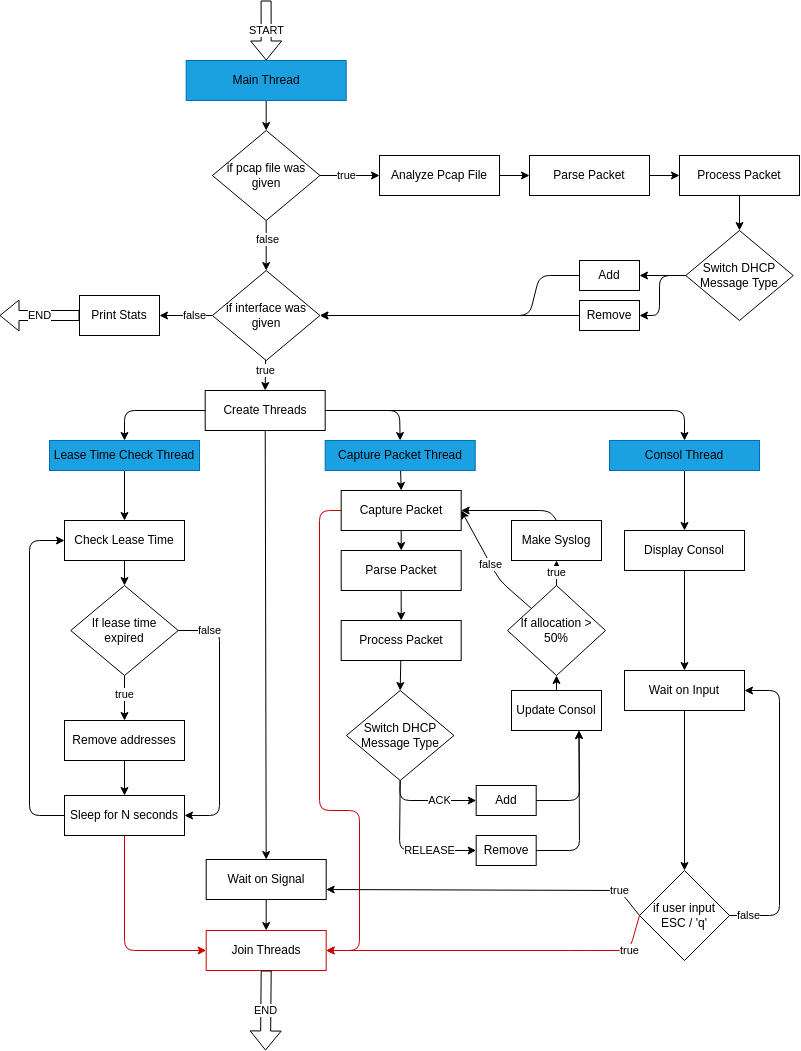
\includegraphics{../images/dhcp-stats-design.png}}
    \end{center}
    \caption{Graph of program operations}
    \label{figure:dhcp-stats-design}
\end{figure}

\noindent Figure \ref{figure:dhcp-stats-design} outlines the primary operations of the program. It is important to note that the first step is
processing the program arguments. Only after the argument processing stage, the operations detailed in figure \ref{figure:dhcp-stats-design} are executed.

\bigskip

\noindent When a pcap file is specified, it takes precedence in processing. If an Internet interface is also provided, the program begins network monitoring 
on the specified interface after processing the file. If the Internet interface is not specified in the program's arguments, the program outputs statistics to 
stdout and finishes its operation. Before the packet capture starts, three threads are initiated. The \texttt{Lease Time Check Thread} periodically verifies lease 
time expiration for all allocated IP addresses. If the lease time has expired for an IP address, it is removed from the list of allocated addresses.
The \texttt{Console Thread} displays statistics in the console. Upon entering \texttt{q} or \texttt{ESC} into the console, a stop signal is sent, prompting the program to finish.
The \texttt{Capture Packet Thread} captures and processes packets, executing actions such as adding or removing an IP address from the statistics based on the packet DHCP message type. 
After each add/remove action, the method in the 'ConsolLog' class is invoked, updating the displayed data.
The red arrows indicate the places from where the threads are connected again after receiving the stop signal.


\section{Implementation description}

\begin{figure}[ht]
    \begin{center}
        \scalebox{0.5}{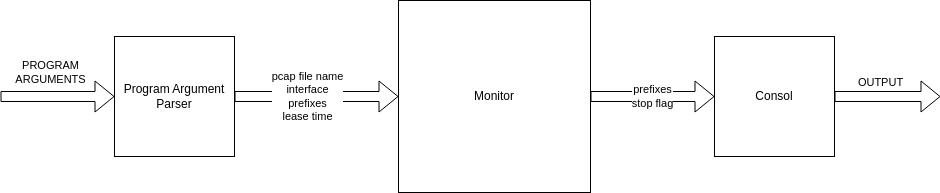
\includegraphics{../images/dhcp-stats-comp.png}}
    \end{center}
    \caption{DHCP-stats application components}
    \label{figure:dhcp-stats-comp}
\end{figure}

This program consists of three main components:

\begin{itemize}
    \item \textbf{ArgParser: } This component is responsible for processing program arguments. It contains a \texttt{parse()} method that processes and returns the arguments entered during the program's startup. Additionally, this component validates whether all required arguments were provided and checks the validity of the arguments.
    \item \textbf{DHCPMonitor: }Serving as the backbone of the application, this component handles network monitoring, DHCP packet processing, and pcap file analysis (if specified in the program arguments). The \texttt{analyze()} method first processes the pcap file and subsequently monitors the network and processing packets on the chosen interface. The more detailed description of the Monitor is in figure \ref{figure:dhcp-stats-design}
    \item \textbf{ConsolLog: }This component manages the display of information related to selected prefixes. If a prefix exceeds the limit of 50\% of allocated addresses, ConsolLog records this information in the syslog.
\end{itemize}


\noindent Each prefix is represented by an instance of the IPv4Prefix class. This class contains methods for working with prefixes and stores the number of 
allocated addresses for a given prefix. An IPv4 address is represented as a 32 bit unsigned integer (\verb|unit32_t|). The \texttt{UINT2IP()} and \texttt{IP2UINT()} methods are used to 
convert IPv4 addresses into string form and back.

\section{Application brief}

\noindent This program allows retrieving information about network prefix utilization in terms of allocated IP addresses. 
Upon execution, the program begins monitoring DHCP traffic on the selected interface or processes a specified pcap file.
It generates statistics on the utilization of the network prefix provided in the command line.
When the prefix is filled to more than \textbf{50\%}, the tool notifies the administrator and creates a log using a syslog server.


\subsection{Functionality}

\noindent This application specifically monitors DHCP acknowledgment and DHCP release packets. When processing a DHCPACK packet, 
a new IP address is allocated within the corresponding prefixes. Upon receiving a DHCPRELEASE packet, the sender's (source) IP address is removed from the list of allocated addresses.
If DHCP acknowledgment is received for already allocate IP address, then only lease time of IP address is updated.

\bigskip

\noindent The application requires either a pcap file that it analyzes or an network interface on which it will monitor DHCP packets. 
If both the pcap file and the network interface are specified in the program arguments, then after processing the pcap file, the application continues processing packets on the specified network interface.

\bigskip

\noindent The lease time is checked for packets in the pcap file only when the network interface is specified in the program arguments. 
Lease time for network communication is always checked. 
This approach ensures that the monitored communication statistics remain current. Additionally, it allows for the analysis of older DHCP communication statistics.
If the lease time of the IP address has expired, the IP address is removed from the list of allocated IP addresses.


\subsection{Limitations}

\noindent If the client responds to the DHCPACK message with a DHCPDECLINE message, the IP address will still remain allocated. 
Consequently, the prefixes associated with this address will continue to include it in the statistics.

\bigskip

\noindent If a DHCPNAK message is sent in response to a DHCPREQUEST message intended to renew the lease time of the IP address, the IP address will persist in allocation. 
Consequently, the prefixes to which this address belongs will continue to include it in the statistics.

\bigskip

\noindent If the DHCP packet contains the \texttt{option overload}, incorrect processing of the packet may occur, 
especially if the \texttt{message type} and \texttt{lease time} options fall outside the standard options field in the DHCP packet.

\bigskip

\noindent Logs and warning messages are created only if network interface is specified. This is because it make no sense to create logs or send warning messages
during just pcap file analysis. However, if network interface is specified in program arguments then warning notifications from pcap file analysis are 
printed to \texttt{stdout} and notifications from network analysis are printed to program \textbf{console}.

\bigskip

\noindent This program can proccess packets that are structured only like this:\newline
\texttt{Ethernet header} + \texttt{IPv4 header} + \texttt{UDP header} + \texttt{DHCP header}.


\subsection{Requirements}

\begin{itemize}
    \item C++ compiler
    \item Standard C++ libraries
    \item pcap library
    \item NCURSES library
    \item Syslog library
\end{itemize}


\section{Program arguments}

\texttt{./dhcp-stats \dots}\\


\noindent To print information about porgram usage use single argument \texttt{-h} or \texttt{---help}

\noindent Required program arguments:

\begin{itemize}
    \item \texttt{[-i <interface> | ---interface <interface>]}: Specifies the network interface where the dhcp-stats tool will monitor DHCP packets. If a single \texttt{-i | ---interface} argument is provided, the application will list available interfaces
    \item \texttt{[-r <pcap-file> | ---read <pcap-file>]} Pcap file from where dhcp-stats tool can read previously monitored DHCP traffic
    \item \texttt{<ip-prefix> [ <ip-prefix> [ ... ]]} IPv4 prefixes that will be monitored
\end{itemize}

\bigskip

\noindent Optional program arguments:

\begin{itemize}
    \item \texttt{[-t <seconds> | ---lctime <seconds>]} Frequency of lease time check for monitored IP addresses in seconds (default is 60 seconds)
\end{itemize}



\noindent\Large{\textbf{Example :}}

\noindent\texttt{\small./dhcp-stats -r dhcp.pcap -i eth0 -t 30 192.168.1.0/24 10.0.0.0/8\normalsize}\\
\noindent\texttt{\small./dhcp-stats -r dhcp.pcap 172.16.1.0/28 \normalsize}\\
\noindent\texttt{\small./dhcp-stats -i eth0 172.16.1.0/28 10.1.1.1/24\normalsize}\\
\noindent\texttt{\small./dhcp-stats -i \normalsize}
\noindent\texttt{\small./dhcp-stats -h \normalsize}

\noindent


% Literature
\newpage

\bibliographystyle{enplain.bst}
\renewcommand{\refname}{Literature}
\bibliography{manual}

\end{document}
